%% ITAT 2026 / CEUR-WS submission
\documentclass[]{ceurart}

\sloppy
\usepackage{listings}
\lstset{breaklines=true}
\usepackage{amsmath,amssymb}
\usepackage{booktabs}
\usepackage{tikz}
\usetikzlibrary{positioning, arrows.meta}

\begin{document}

\copyrightyear{2026}
\copyrightclause{Copyright for this paper by its authors.
  Use permitted under Creative Commons License Attribution 4.0
  International (CC BY 4.0).}

\conference{ITAT 2026: Information Technologies -- Applications and Theory,
  September 25--29, 2026, Vr\v{s}atec, Slovakia}

\title{A Pipeline Toward an Automated Conjecturing-Refuting-Formalizing-Proving Loop for Graph Theory}



\author[1]{J\'an Pastorek}[%
email=jan.pastorek@fmph.uniba.sk,
orcid=0000-0001-8237-1275,
]
\cormark[1]
% \author[1]{Samuel Varchol}[%
% email=varchol3@uniba.sk,
% ]
% \author[1]{Vladim\'ir Jan\v{c}\'ar}[%
% email=jancar12@uniba.sk,
% ]
\address[1]{Department of Applied Informatics, Comenius University in
  Bratislava, Bratislava, Slovakia}

% \cortext[1]{Corresponding author.}

\begin{abstract}
  We report on our ongoing project to develop a computational pipeline for an automated
  graph-theoretic conjecturing-refuting-formalizing-proving system. Generation is counterexample-guided: a \textsc{Graffiti3} generator (the native nonlinear engine of the TxGraffiti package) proposes inequalities over a small seed
  of a few hundred graphs that grows only by hard counterexamples. We add four components that,
  together, alter the
  nature of the output: (i) a refutation dataset of $\sim\!348{,}000$
  graphs unioning the complete House of Graphs invariant export, the exhaustive census of all connected
  graphs on at most nine vertices, and several special extremal graph families
  (strongly regular, minimal Ramsey, Cayley, cages, barbells, lollipops, spiders, etc.), augmented by on-demand class-aware random models (random-regular, $G(n,p)$, random trees and random bipartite graphs), against which every candidate conjecture is attacked; (ii) a \emph{novelty filter} of $203$ classical theorems known from literature
  and trivial theorems closed under transitive composition and linear
  identity substitution, which decides whether a candidate is implied by them; (iii) a \emph{counterexample search stage} to find counterexamples to surviving conjectures; and (iv) an \emph{autoformalization stage} that translates surviving conjectures into Lean~4 \cite{moura2015lean} statement skeletons, every candidate proof kernel-verified against a pinned \texttt{mathlib4} and our custom invariant preamble. On the cluster we attempt the simplest machine-generated survivors with two state-of-the-art neural provers---\textsc{DeepSeek-Prover-V2-671B} (served with vLLM) and the Lean-specialised \textsc{OProver-32B}---but in single-shot whole-proof mode neither verifies any survivor: the conjectures are expressed over \emph{custom} graph invariants outside the provers' training distribution, and closing the conjecture$\to$proof loop end-to-end remains open. Multi-round agentic proving with compiler feedback and invariant-definition grounding is under evaluation.
\end{abstract}

\begin{keywords}
  automated conjecturing \sep
  automated theorem proving \sep
  graph theory \sep
  counterexample search \sep
  TxGraffiti
\end{keywords}

\maketitle

\section{Introduction}

Computer-assisted discovery of mathematical results and conjectures has a long history and with the advent of artificial intelligence and high-performance computing, it
is increasingly recognized as valuable in the mathematical community.

Computer-assistance in this area can be roughly classified into four corresponding areas based on the research stage it assists: \emph{conjecturing} new statements based on a finite database, \emph{refuting} them by searching for counterexamples, \emph{formalizing} them into a rigorous language, and ultimately \emph{proving} them in a formal system.

Automated conjecturing in graph theory has a forty-year history, from
Fajtlowicz's \textsc{Graffiti}~\cite{fajtlowicz1988conjectures,wiki2026graffiti,larson2002intelligent} and
DeLaVi\~na's \textsc{Graffiti.pc}~\cite{delavina2002graffitipc,delavina2004history}
to the \textsc{AutoGraphiX}/\textsc{GraPHedron} programme of Aouchiche,
Caporossi, Hansen, and M\'elot~\cite{aouchiche2009variable,caporossi2004graphedron,melot2008facet} and,
more recently, Davila's \textsc{TxGraffiti}~\cite{davila2024automated,caro2022txgraffiti}
and \textsc{The Optimist}~\cite{davila2024optimist}, Larson's Dalmatian-based
\textsc{Conjecturing}~\cite{larson2016dalmatian,larson2017automated} and
\textsc{Graffiti}$^3$~\cite{davila2026graffiti3}, and the polyhedral
\textsc{PHOEG} system~\cite{bonte2026phoeg}. These systems propose inequalities
between graph invariants---$\alpha(G)\le\nu(G)$, $\chi(G)\le\Delta(G)+1$, and
so on---by fitting candidate bounds to a finite database of graphs and retaining and sorting only those that pass a set of filters and heuristics. Many resulting conjectures 
have become theorems; some have been refuted by hand or by machine
search, see for instance~\cite{brewster1995computational,larson2017automated,jooken2025computer}.

A practitioner who reimplements such a system quickly encounters five possible failure modes.
First, a candidate can hold on every graph in a finite database yet be
\emph{false in general}: the database simply lacks the structure that breaks
it. Second, the system can produce a candidate that is \emph{true but known}, already recorded in the literature. Third, the system can produce a candidate that is \emph{true but trivial}, resulting in an ``avalanche of triviality''. Fourth is the \emph{monster conjecture}: a single
conjecture that overfits the table by accumulating many terms and constants
(producing unnecessarily complex bounds such as $\alpha\le 0.31\,\Delta+0.42\,\nu-0.07\,m+1.8$).
Fifth, the system can ``discover'' a counterexample
to a well-established conjecture, which almost always signals an error in an
invariant routine or a misread statement rather than a result. The first and the last failure
modes are about \emph{trust}: a generated inequality that ``holds'' and a
verified ``counterexample'' are each only as reliable as the data and invariant computations behind them. The second and the third failure modes are about \emph{novelty}: a candidate that is true but known, or true but trivial, is mathematically uninteresting and of little value to the practitioner. All of these failure modes are addressed in our pipeline by the adversarial counterexample search, the novelty filter, and the selection heuristics. 

To address the first and fourth failure modes---false bounds and overfitting---a robust refutation engine is required. Computational methods used for searching for (counter)examples of graphs have been recently summarised in a review article of Jorik Jooken~\cite{jooken2025computer}. Among others, the methods include exhaustive search with branch and bound, randomised search, and heuristic search. More recently, deep reinforcement learning has been applied to refute several conjectures \cite{wagner2021constructions}.

Lastly, there is a growing body of recent work on autoformalization and automated theorem proving especially in Lean, including for graph theory, see for instance \cite{wu2022autoformalization,mavani2026chipfiring,nader2026gtbench,kalfus2026ramsey,zhang2026leanmarathon,deepseek2025prover}. However, although we recently found in \cite{davila2026graffiti3} certain indications in this direction, to the best of our knowledge there is no existing system that integrates automated conjecturing, refuting, formalizing, and proving in a closed loop for graph theory.

In this paper, we describe and report on the development of such a computational system \textsf{AutoGraphForge} that aims to combine (i)-(iv) in a pipeline. The first two stages are often combined into a \emph{generate-refute} loop, where conjectures are generated and then tested against a database of known graphs and invariants, with counterexamples being added to the database for future iterations. The last two stages are often combined into a \emph{formalize-prove} loop, where conjectures are translated into a formal language Lean and then attempted to be proved using automated theorem provers.

Our current contributions are:

\begin{enumerate}
  \item We build the first version of the computational pipeline \textsf{AutoGraphForge} and run it on a
  high-performance computing cluster: a multi-round counterexample-guided inductive synthesis
  (generate-refute) loop partitioned into five full-node SLURM jobs
  (each partitioning the invariant list), followed by a merge and a GPU proving stage that serves
  \textsc{DeepSeek-Prover-V2-671B} with vLLM to kernel-verify the simplest survivors. The end-to-end
  proving results of this scaled run are still in progress; the proving results reported in this
  paper are those of the in-process $7$B model (\S\ref{sec:refute}).
  \item We build a refutation dataset of $348{,}207$ graphs (carrying up to
  $59$ exactly-computed invariants), combining the complete House of Graphs (HoG)~\cite{coolsaet2023house} export and many other extremal graph families, including the strongly-regular, minimal-Ramsey,
  Cayley, cage, cograph, and minimally-rigid families, barbells, lollipops, spiders, and complements of
  triangle-free graphs, together with on-demand class-aware random models. Generation itself runs over a small evolving
  seed (a few hundred graphs), not the full dataset.
  \item A novelty filter of $203$ classical or trivial theorems
  (\S\ref{sec:heuristics_related}), closed under transitive composition of $f\le g$
  relations and under linear identity substitution (e.g. the regular-graph
  identity $\Delta=\delta=2m/n=\rho=\mathrm{degeneracy}$, K\"onig's $\nu=\tau$,
  Gallai's $n=\alpha+\tau$), implemented as a small linear-program feasibility
  test. The filter is a \emph{sound but incomplete} implication test: a positive verdict certifies
  that a candidate is genuinely implied by the tabled theorems and identities (not merely that it
  matches a template), while a candidate that is in fact derivable through inter-invariant relations
  not encoded in the table may still pass through as ``novel.''
\item A permanent \emph{adversarial verification stage} (\S\ref{sec:adv}):
  every candidate is tested against on-demand structure-targeted datasets (\S\ref{sec:data})---a
  parametric/atlas dataset (barbells, lollipops, spiders, class generators, complements of
  triangle-free graphs) and a class-aware random-models dataset---constructed to break loose bounds;
  in the single-pass run reported in \S\ref{sec:adv} these materialised $1{,}142$ and $219$ graphs
  respectively. This stage runs
  first in the falsification loop and stores found counterexamples back into
  the dataset.
\item A validated counterexample-search engine
  (\S\ref{sec:engine}) that includes among others recent state-of-the-art methods such as probabilistic search using the cross-entropy method and Monte Carlo methods. To validate it we reproduced the refutation of a number of conjectures and exhaustively verified a
  range of open conjectures (\S\ref{sec:engine}).
% \item A separate, exploratory integration of the \textsc{Conjecturing} package
\end{enumerate}

We note that our system is not built from scratch but is built upon existing packages, frameworks and methodologies present in the state-of-the-art literature on each of the three areas of conjecturing, refuting, and formalizing and proving. In particular, the conjecture generation is built on top of TxGraffiti; the counterexample search engine is built upon recent state-of-the-art methods such as probabilistic search using the cross-entropy method and Monte Carlo methods described in \cite{jooken2025computer}; and the formalization and proving layer is built upon recent autoformalization methods and automated theorem provers, specifically Lean~4 with \texttt{mathlib4} as the target language and the \textsc{DeepSeek-Prover-V2} automated prover~\cite{deepseek2025prover}.

\section{Preliminaries}
\label{sec:preliminaries}

All graphs in this paper are considered finite and simple. For a graph $G$ we write
$n=n(G)$ for its \emph{order} (number of vertices) and $m=m(G)$ for its
\emph{size} (number of edges). We use standard invariant symbols throughout:
maximum and minimum degree $\Delta,\delta$, average degree $2m/n$, and
\emph{degeneracy}; independence number $\alpha$, matching number $\nu$,
vertex-cover number $\tau$, clique number $\omega$, chromatic number $\chi$,
chromatic index $\chi'$, domination number $\gamma$, and independent-domination
number $i$; vertex- and edge-connectivity $\kappa$ and $\lambda$; radius
$\mathrm{rad}$, diameter $\mathrm{diam}$, and triangle count $\mathrm{tri}$; and
the largest adjacency eigenvalue, or \emph{spectral radius}, written $\lambda_1$
and equivalently $\rho$ ($\lambda_1=\rho$; neither to be
confused with the edge-connectivity $\lambda$). The \emph{barbell} $K_a\!-\!K_b$ denotes two disjoint cliques joined by a bridge (a standard, informal notation).
On a regular graph $\rho$ equals the common degree, giving the identity
$\Delta=\delta=2m/n=\rho$. The clique-cover number---the minimum number of
cliques covering $V(G)$, equivalently $\chi(\overline G)$---is written
$\overline{\theta}$ throughout. 

\section{The AutoGraphForge Architecture}

\subsection{System overview}
\label{sec:pipeline-fig}
At a high level, \textsf{AutoGraphForge} is a continuous, self-critical loop
(Figure~\ref{fig:pipeline}) that couples generation, selection heuristics,
refutation search, and a formalization/proving layer, in the spirit of the
competing optimist/pessimist ``GraphMind'' architecture of
\textsc{The Optimist}~\cite{davila2024optimist}. Candidate conjectures are scored
and ranked, then aggressively tested by the refutation engine (the
``pessimist''); only statements that survive multiple rounds advance to
autoformalization, proving, and human review, while every counterexample feeds
back into the knowledge base. The remaining sections detail each stage in turn:
the data (\S\ref{sec:data}), generation and selection (\S\ref{sec:theory-selection}),
refutation (\S\ref{sec:refute}), and formalization and proving
(\S\ref{sec:formalize-prove}).

\begin{figure}[htbp]
    \centering
    \resizebox{\columnwidth}{!}{%
    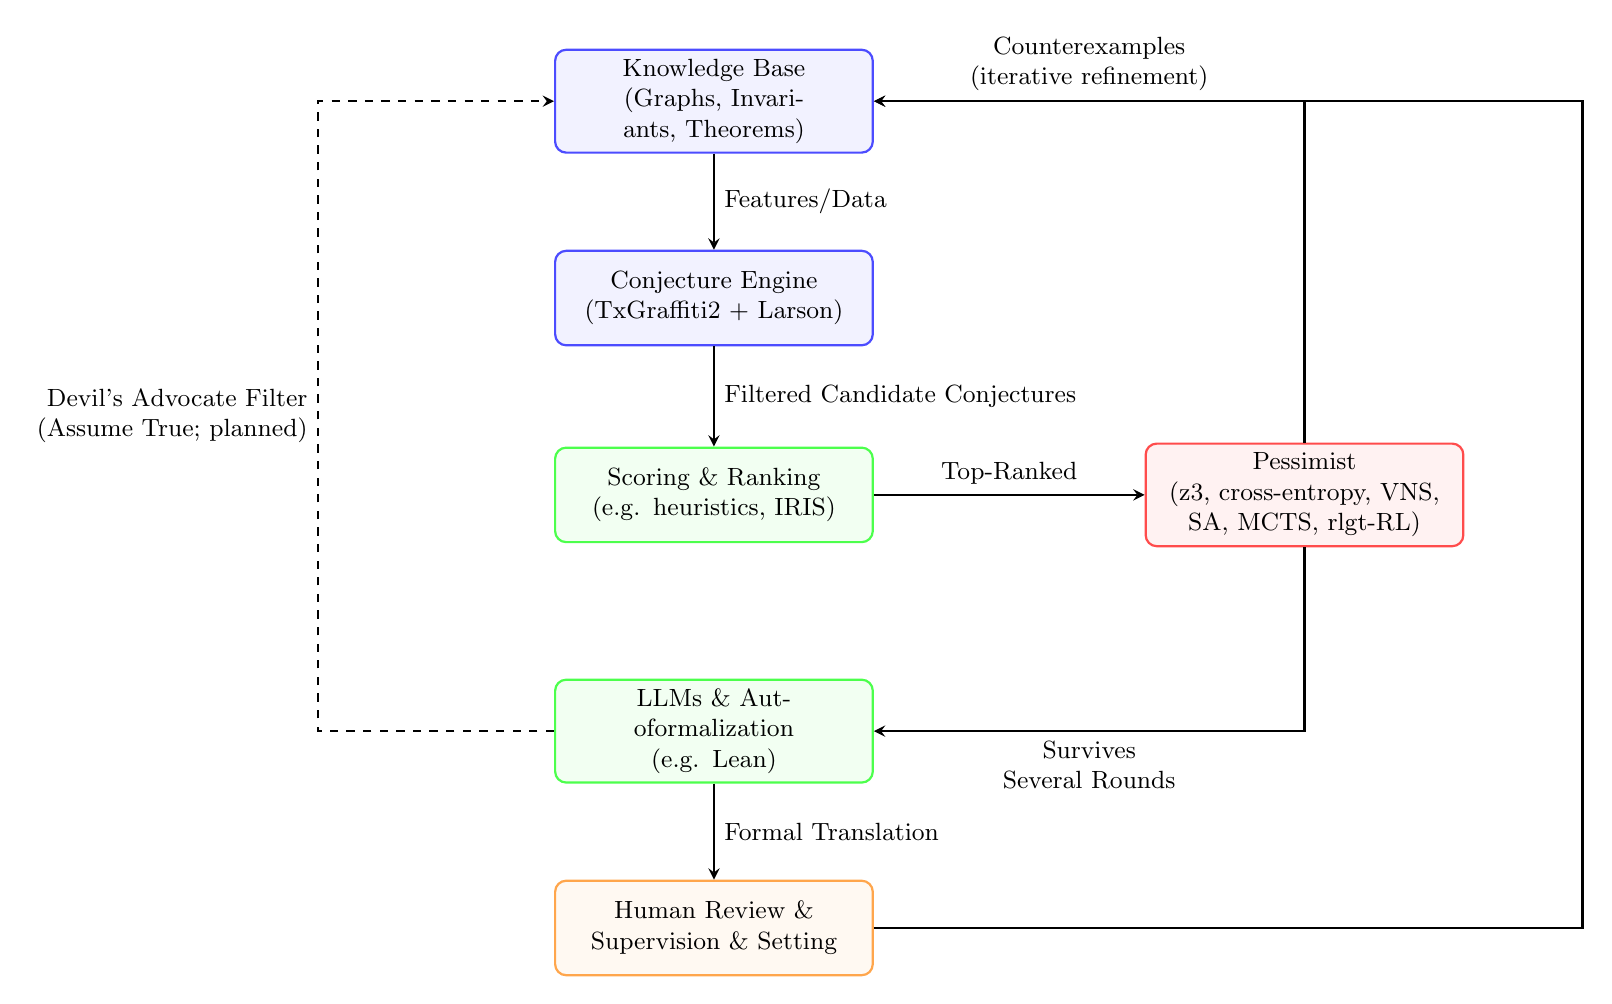
\begin{tikzpicture}[
        box/.style={draw=blue!70, fill=blue!5, rectangle, rounded corners, minimum width=3.8cm, minimum height=1.2cm, align=center, text width=3.8cm, thick},
        pessimist/.style={draw=red!70, fill=red!5, rectangle, rounded corners, minimum width=3.8cm, minimum height=1.2cm, align=center, text width=3.8cm, thick},
        extension/.style={draw=green!70, fill=green!5, rectangle, rounded corners, minimum width=3.8cm, minimum height=1.2cm, align=center, text width=3.8cm, thick},
        human/.style={draw=orange!70, fill=orange!5, rectangle, rounded corners, minimum width=3.8cm, minimum height=1.2cm, align=center, text width=3.8cm, thick},
        arrow/.style={->, thick, >=stealth},
        font=\small
    ]
    % Nodes
    \node[box] (kb) at (0, 0) {Knowledge Base \\ (Graphs, Invariants, Theorems)};
    \node[box] (engine) at (0, -2.5) {Conjecture Engine \\ (TxGraffiti2 + Larson)};
    \node[extension] (iris) at (0, -5) {Scoring \& Ranking \\ (e.g. heuristics, IRIS)};
    \node[pessimist] (pessimist) at (7.5, -5) {Pessimist \\ (z3, cross-entropy, VNS, SA, MCTS, rlgt-RL)};
    \node[extension] (autoformal) at (0, -8) {LLMs \& Autoformalization \\ (e.g. Lean)};
    \node[human] (human) at (0, -10.5) {Human Review \& Supervision \& Setting};

    % Main flow arrows
    \draw[arrow] (kb) -- node[right] {Features/Data} (engine);
    \draw[arrow] (engine) -- node[right] {Filtered Candidate Conjectures} (iris);
    \draw[arrow] (iris) -- node[above] {Top-Ranked} (pessimist);

    \draw[arrow] (human.east) -- ++(+9,0) |- (kb.east);

    % Loop back from Pessimist
    \draw[arrow] (pessimist.north) |- node[above, pos=0.75, align=center] {Counterexamples \\ (iterative refinement)} (kb.east);

    % Success path from Pessimist
    \draw[arrow] (pessimist.south) |- node[below, pos=0.75, align=center] {Survives \\ Several Rounds} (autoformal.east);

    % Autoformalization to Human
    \draw[arrow] (autoformal) -- node[right] {Formal Translation} (human);

    % Devil's Advocate Filter
    \draw[arrow, dashed] (autoformal.west) -- ++(-3,0) |- node[left, pos=0.25, align=right] {Devil's Advocate Filter \\ (Assume True; planned)} (kb.west);
    \end{tikzpicture}}
    \caption{The integrated automated mathematical discovery pipeline.
    Conjectures are generated, immediately scored and ranked (heuristics, IRIS),
    and then aggressively tested by the refutation engine (the Pessimist:
    adversarial dataset plus z3/cross-entropy/VNS/SA/MCTS/rlgt search). Only conjectures surviving
    multiple rounds of refutation are passed to LLMs for autoformalization; found
    counterexamples are fed back into the knowledge
    base. The dashed line is the planned Devil's Advocate filter (future work; see
    the Conclusion), where surviving
    conjectures would be assumed true to constrain future generation, before advancing
    to final human review.}
    \label{fig:pipeline}
\end{figure}
\subsection{Invariants and the database}
\label{sec:data}

Trust in generated inequalities is bounded by trust in the data. We combine
several sources. The HoG export~\cite{goedgebeur2022introduction,coolsaet2023house} provides $28{,}859$ graphs with $\sim\!28$
pre-computed invariants each (treewidth, feedback-vertex-set number, spectral
data, vertex cover, girth, \dots), parsed directly so that nothing is
recomputed; values marked \texttt{undefined}, \texttt{infinity}, or
\texttt{Computation time out} are treated as missing. Database also contains every connected graph on $2\le n\le 9$ vertices ($273{,}192$ graphs)
through an exact invariant list and a set of computed graph-class flags
(triangle-free, cubic, claw-free, cograph, split, outerplanar,
self-complementary, Hamiltonian, well-covered). We also used the HoG meta-directory to collect cograph, minimal-Cayley, cage,
minimal-Ramsey, strongly-regular (Spence), and minimally-rigid graph families. The
union contains $348{,}207$ graphs and up to $59$ exactly-computed invariant columns. This static
dataset is one refutation resource; alongside it the refuter draws on two further datasets computed
on demand with the exact list: parametric families (barbells, lollipops,
spiders, $k$-trees, line graphs, Delaunay graphs, $\alpha=2$ complements, \dots) and random graph models (random-regular, Erd\H{o}s--R\'enyi $G(n,p)$, random trees,
and random bipartite graphs, several per (class,\,order)), so that refutation probes the average invariants corresponding to each class and not only structured or special witnesses. Conjecture
\emph{generation}, by contrast, runs over a small initial seed described in
\S\ref{sec:pipeline-arch}.

\paragraph{Backend invariant calculation.} A single backend,
\textsc{GraphCalc}~\cite{davila2025graphcalc}, is designated \emph{canonical}:
every value that enters the store is its exact computation, or left empty. An
independent \texttt{networkx}~\cite{hagberg2008networkx} list is registered purely as a cross-check, and
a \texttt{crossvalidate} script compares the two on sample graphs before any build is
trusted---reproducing the zero-mismatch result below, now as an automated
precondition rather than a one-off audit. The two connectivity invariants
\textsc{GraphCalc}~lacks ($\kappa,\lambda$) are sourced from \texttt{networkx}
and likewise blanked when unavailable; no value is ever silently approximated by
a second backend.

\paragraph{Validation against an authoritative reference.} We verified computation of invariants of \textsc{GraphCalc} against the independently-computed HoG values on $2{,}500$
graphs: for every shared invariant
($\chi,\alpha,\omega,\gamma,\nu,\Delta,\delta,\kappa,\lambda,\mathrm{diam},
\mathrm{tri}$, and the booleans) there were \emph{zero} mismatches.

\subsection{Conjecture generation as theory selection}
\label{sec:theory-selection}
Treat the examples and counterexamples as rows of a common invariant table $T$,
whose numerical columns embed the objects as a point cloud in $\mathbb{R}^k$ (where $k$ is the number of invariants)---the
\emph{invariant cloud}. A linear grammar of conjectures consists of halfspaces
$\sum_i a_i f_i(G)\le c$ (with $a_i, c \in \mathbb{R}$) that must hold for every row of the current snapshot.
The convex hull of the cloud makes the core difficulty geometric: there are
infinitely many snapshot-true inequalities (any halfspace whose boundary lies
above the hull), but only the \emph{facets}---tight on at least one extremal
object---carry information, and no single inequality is ``the best.'' A practical
system is therefore not fitting one predictor but choosing a \emph{budgeted,
nonredundant} theory: a small library of cuts that each strengthen the current
envelope somewhere. Our generation and selection layers (\S\ref{sec:theory-selection})
implement exactly this budget. 

This builds on three distinct paradigms that have emerged for searching the space of graph-theoretic
inequalities. \emph{Algebraic expression trees}, used by \textsc{Graffiti}, build
candidate conjectures as rooted trees of invariants combined by unary and binary
operations (sums, products, square roots), and enumerate candidates by
exhaustive or heuristic tree search. \emph{Linear and mixed-integer programming},
used by \textsc{TxGraffiti}~\cite{davila2024automated,caro2022txgraffiti},
\textsc{The Optimist}~\cite{davila2024optimist}, and
\textsc{Graffiti}$^3$~\cite{davila2026graffiti3}, instead solves an
optimisation model over a precomputed tabular dataset: by minimising the
distance between a target invariant and a linear combination of others, the
tightest possible bound is found without enumeration. The
\emph{polyhedral/geometric} approach of \textsc{GraPHedron}~\cite{melot2008facet,caporossi2004graphedron} and
\textsc{PHOEG}~\cite{bonte2026phoeg,christophe2008linear} embeds each graph as a
point in invariant space and reads off conjectures as facets of the resulting
convex hull; this produces the \emph{complete} set of optimal linear
inequalities for those invariants and makes optimality a geometric certificate.

The methods are released as a single package, \textsf{AutoGraphForge},
that takes \textsc{TxGraffiti2}~\cite{davila2024automated} as its foundation. The canonical representation of a
conjecture is TxGraffiti2's own \texttt{Conjecture} object, and every subsequent component---the implication-deciding novelty filter, the
selection heuristics, and the refutation engine---is built to take these
native objects directly.

\subsubsection{Architecture and linear generation}
\label{sec:pipeline-arch}
We build upon TxGraffiti2's native convex-hull and ratio generators and its implementation of the Dalmatian dominance filter, meaning the generation logic operates directly on Pareto-optimal frontiers of non-dominated, tight bounds without redefining them. Invariants
are supplied by \textsc{GraphCalc} (\S\ref{sec:data}). In the runs reported here the generator is
\textsc{Graffiti3}~\cite{davila2026graffiti3} (the native nonlinear conjecturing
engine of the TxGraffiti package) which additionally mines ratio,
product, $\sqrt{\cdot}$ and $\log$ bounds together with \emph{Sophie} sufficient-conditions over
the seed's $59$-invariant \textsc{GraphCalc} list. 

Generation begins from the TxGraffiti \emph{expressive graphs} (a curated default dataset) and grows only by hard witnesses. The single-round figures quoted in \S\ref{sec:dynamics} come from
an earlier one-pass run; the HPC run (\S\ref{sec:dynamics}) instead iterates for up to $25$
generate--refute rounds, stopping early if it cannot find counterexamples to any conjectures or at a
wall-clock budget, so that each round conjectures over a strictly larger,
counterexample-hardened seed.

\subsubsection{Product and ratio conjectures}
\label{sec:products}
Ratios reduce to linear bounds ($f/g\le c\iff f\le cg$), so the genuinely new
expressive power is in products. The product sweep rediscovered the classical
product theorems---$n\le\alpha\chi$ (Gallai~\cite{gallai1959uber}),
$n\le\gamma(\Delta+1)$ and
$n\le\alpha(\Delta+1)$ (greedy/domination)---which is precisely the desired
correctness signal, together with provable handshake bounds such as $\alpha\delta\le
m$ (the edges incident to an independent set number at least $\alpha\delta$).
After adversarial filtering, the product remainder is, like the linear remainder,
dominated by known or provable bounds.


\subsection{Novelty filtering and dominance heuristics}
\label{sec:heuristics_related}
Without aggressive filtering, conjecture systems suffer a ``combinatorial
explosion,'' generating thousands of trivial or redundant statements. \emph{Simplicity Over Complexity}: While optimization models can handle bounds with many invariants simultaneously, based on an Ockham's razor principle, bounds with both fewer invariants, and arithmetic and logical operations are preferred. \emph{Strongest-Conjecture principle} requires that the system assert only the
tightest bound for which no counterexample is known; this is the formal basis of
the Dalmatian dominance filter and the polyhedral facet approach alike.
The \emph{Dalmatian heuristic} (dominance), due to Fajtlowicz and revisited by
Larson and Van~Cleemput~\cite{fajtlowicz1988conjectures,larson2016dalmatian},
discards a candidate whenever some accepted conjecture is never weaker and
sometimes strictly tighter; this is the primary filter used throughout our pipeline
(\S\ref{sec:theory-selection}), alongside a linear programming novelty filter that decides whether an inequality is a trivial combination of already known mathematical relations (\S\ref{sec:heuristics_related}). We also utilise the \emph{Sophie heuristic}, which shifts from producing a numeric bound to identifying a Boolean property that fully characterises all sharp graphs, converting an inequality into a structural characterisation.

Discovering a candidate inequality is only part of the task: the system must also
decide whether the inequality is genuinely new or merely a combination of
already-known relations.

Suppose the system generates a candidate inequality
\[
    f \le R(g),
\]
where $f$ is a target invariant (for example, the independence number) and $R(g) \triangleq \sum_i c_i g_i + c_0$ is a linear combination of other invariants $g_i$, with $c_i, c_0 \in \mathbb{R}$. Before accepting it, the system tests it against a curated library of known theorems that bound the same target invariant ($f \le B_1(g)$, $f \le B_2(g)$, and so on, where each $B_j(g)$ is a known affine bound on $f$).

The candidate is declared \emph{known} (redundant) if it is implied by a convex combination of these theorems. Assigning a non-negative weight $w_j$ to each $B_j(g)$ with $\sum_j w_j = 1$ yields the aggregate bound $f \le \sum_j w_j B_j(g)$. If this aggregate is at least as tight as $R(g)$, the candidate is redundant; equivalently, the difference between the candidate and the aggregate is non-negative everywhere:
\[
    R(g) - \sum_j w_j B_j(g) \ge 0.
\]

\subsubsection*{The non-negativity certificate}

To certify that this difference is non-negative, we express it identically as a sum of terms that are individually non-negative. We seek weights $w_j \ge 0$, non-negative slack variables $s_i, t \ge 0$, and free multipliers $\mu_k \in \mathbb{R}$ such that the following identity holds for all $g$:
\[
    R(g) - \sum_j w_j B_j(g) = \sum_i s_i(g_i - L_i) + \sum_k \mu_k E_k(g) + t.
\]

The right-hand side is composed of terms each guaranteed to be non-negative:
\begin{itemize}
    \item \emph{Safe lower bounds} $s_i(g_i - L_i)$: every invariant $g_i$ has a known minimum value $L_i$, so $(g_i - L_i) \ge 0$; multiplying by a non-negative slack $s_i$ preserves non-negativity.
    \item \emph{Class identities} $\mu_k E_k(g)$: structural relations $E_k(g)=0$ that hold identically on a graph class $P_k$, so multiplying by any free multiplier $\mu_k$ does not affect non-negativity. Crucially, soundness requires that $E_k$ strictly vanish on the whole domain the candidate is quantified over, so each identity is \emph{class-gated}: it is admitted only when the candidate's hypothesis class is $P_k$ or a subclass of it. For an \emph{unconditioned} candidate, only \emph{universal} identities (those with $P_k$ = all graphs, e.g.\ Gallai's $n=\alpha+\tau$) are available; a class-restricted identity such as K\"onig's $\nu=\tau$ (bipartite only) is never used to declare an unconditioned candidate known, which would otherwise be an unsound false positive.
    \item \emph{Constant slack} $t$: a non-negative scalar absorbing the residual constant.
\end{itemize}

Because the invariants $g_i$ are treated as independent symbolic variables, matching the coefficient of each $g_i$ on both sides reduces the problem to a system of linear equations. Verifying redundancy therefore reduces to a linear-programming (LP) feasibility test: if the solver finds weights and slacks satisfying the identity, the candidate is provably a structural consequence of the tabled theorems and is discarded.

The table holds $203$ entries after closing the simple $f\le g$
relations under transitivity; the class-gated identity multipliers $\mu_k$ capture, in one
mechanism, Whitney's connectivity chain $\kappa\le\lambda\le\delta$~\cite{whitney1932congruent}
(all graphs), K\"onig's $\nu=\tau$~\cite{konig1931graphen} (bipartite), and
Gallai's $n=\alpha+\tau$~\cite{gallai1959uber} (all graphs)---each applied only on the class where
it holds. The filter correctly hides, for
example, $\kappa\le\tfrac12\delta+\tfrac12\lambda$.

\subsubsection{Sophie layer: sufficient conditions}
\label{sec:sophie}
Using the \emph{Sophie} heuristic (introduced in \S\ref{sec:heuristics_related}) directly from its \textsc{Graffiti}$^3$ implementation, the same machinery, in its boolean mode, produces \emph{sufficient conditions}
for a graph property rather than numeric bounds: statements
$P_1\wedge\cdots\wedge P_k\Rightarrow Q$ (where $k \ge 1$) built from a
set of boolean predicates (regularity, planarity, claw-freeness, chordality,
$2$- and $3$-connectivity, the Dirac threshold $2\delta\ge n$, vertex
transitivity, even order, \dots) with the logical operators
$\neg,\wedge,\vee,\rightarrow$. Targeting Hamiltonicity and the existence of a
perfect matching, with Dirac's theorem~\cite{dirac1952some} supplied as the
theory and the same
adversarial filter applied, the search recovers genuine theorems---most
strikingly Sumner's result~\cite{sumner1974graphs} that a connected claw-free
graph of even order has a
perfect matching ($\textsf{even order}\wedge\textsf{claw-free}\Rightarrow
\textsf{perfect matching}$)---alongside plausible conditions such as
$\textsf{2-connected}\wedge\textsf{claw-free}\Rightarrow\textsf{Hamiltonian}$
and $\textsf{3-connected}\wedge\textsf{planar}\Rightarrow\textsf{Hamiltonian}$.
That a system rediscovers Sumner's theorem from data, rather than fitting an
artefact, is again the desired correctness signal. In the HPC run these
sufficient-conditions are no longer merely validated at generation time: each
$\textsf{hyp}\Rightarrow\textsf{property}$ is routed through the same tiered
refutation dataset as the inequalities, refuted by any graph on which the
hypothesis relation holds but the property fails (NaN-aware, so a dataset lacking
the property is a coverage miss, never a false refutation). This is what removes
spurious sufficient-conditions such as
$(\textsf{order}\le14)\Rightarrow\textsf{connected}$ that hold across a
connected-only snapshot but are false in general.

\subsection{Iterative refutation and adversarial search}
\label{sec:refute}
Because the target class is infinite and the snapshot is a biased partial view,
``true on the table'' is a statement about present \emph{evidence}, not a
generalisation claim. The proper analogue of a test set is therefore not a
static validation set but an \emph{iterative counterexample search}: an actively targeted
search for objects outside the table on which proposed laws fail. When this search
succeeds, the counterexample is promoted into the table, changing the feasible
space of all subsequent conjectures. This makes conjecturing intrinsically
online---the dynamic-database principle---and it is realised concretely by the
adversarial dataset, the counterexample-search backends, and dynamic re-insertion
of found counterexamples (\S\ref{sec:refute}). Automated discovery depends on this adversarial loop.
The refutation rules of the \textsc{Graffiti} tradition---the \emph{Red Burton rule} (minimising counterexamples), the \emph{TicTac method}, and \emph{Pepper's rule} (treating every machine-generated conjecture as false until counterexamples are exhausted)---were documented by DeLaVi\~na~\cite{delavina2004history}. More recently, Monte-Carlo algorithms~\cite{cazenave2009nested,rosin2011nested} and probabilistic optimization~\cite{wagner2021constructions} have been applied directly to automated refutation (for a review see \cite{jooken2025computer}), building counterexample graphs edge by edge guided by the conjecture's violation margin.

Generation is inexpensive; rejection is the decisive step. Every candidate
that survives novelty and selection is passed to the adversarial stage.

\subsubsection{Adversarial verification}
\label{sec:adv}
A finite database cannot certify a universally-quantified statement. We make
this concrete: the bound $\delta(G)\le\lambda(G)+5$ holds on all $347{,}855$
graphs of the combined dataset on which $\lambda$ is defined, yet is
false---the barbell $K_{10}\!-\!K_{10}$
has $\delta=9,\lambda=1$. The combined dataset simply contains no graph with
$\delta-\lambda>5$.

The adversarial stage therefore tests each candidate against structure-targeted datasets with exact
invariants---generated on demand (\S\ref{sec:data}), materialising $1{,}142$ parametric/atlas graphs
(families) and $219$ class-aware random graphs for the single-pass run quoted below---of
barbells (large $\delta$, small $\lambda$), cliques with sparse tails (high
$\chi/\omega$, low average degree), spiders (large radius, small $\gamma$),
random regular graphs, $k$-trees, line graphs, Delaunay (planar) graphs, and
complements of triangle-free graphs ($\alpha=2$). The linear
artefacts $\delta\le\lambda+5$ and $\chi\le 2m/n+3$ are typically refuted instantly by this collection. The
stage runs first in the falsification loop and stores any counterexample it
finds in a growing dataset, so refutations accumulate across rounds.



\paragraph{Dynamic database.} Any found counterexample is inserted into the database, iteratively
tightening subsequent candidate conjectures in the next rounds. This realises the iterative counterexample search loop of
\S\ref{sec:refute} in code: the feasible region of invariant space
contracts with every refutation, and the same artefact is never proposed twice.

\subsubsection{Counterexample-search backends}
\label{sec:backends}
For conjectures whose counterexamples lie outside any fixed dataset, the system
provides four interchangeable search backends, all sharing a single
``$\mathrm{margin}(G)>0\iff G$ refutes'' interface and tried cheapest-first per
candidate:

\begin{itemize}
  \item \emph{SMT (satisfiability-modulo-theories) encoding} (\textsf{z3}): graph structure is encoded as Boolean edge
    variables; invariant constraints ($k$-colorability, independence set size,
    etc.)\ are expressed as pseudo-Boolean formulae and dispatched to a
    Z3~\cite{demoura2008z3} solver; most effective for graphs on up to $\sim\!10$ vertices.
  \item \emph{Linear cross-entropy} (\textsf{cross\_entropy}): Wagner's
    cross-entropy method~\cite{wagner2021constructions} without a neural network
    --- a per-edge inclusion distribution is sampled in batches, the elite
    fraction with the largest margin is retained, and the distribution is moved
    toward the elite edge frequencies. Gradient-free and cheap.
  \item \emph{Variable-neighbourhood search} (\textsf{vns}): cycles through
    increasingly large flip neighbourhoods ($1$-edge $\to$ $k$-edge $\to$ vertex
    rewiring), accepting any slack-reducing move and restarting from a structured
    seed family (\S\ref{sec:engine}) when trapped in a local minimum.
  \item \emph{Monte-Carlo tree search} (\textsf{mcts}): a standard UCT bandit search
    over edge modifications, guided by the conjecture's negative slack as the rollout reward.
  \item \emph{Simulated annealing} (\textsf{sa}): standard simulated annealing over edge modifications, adopting a temperature schedule to escape local optima.
  \item \emph{Deep reinforcement learning} (\textsf{rlgt-RL}): building on RLGT~\cite{wagner2021constructions}, trains an edge-selection policy guided by the conjecture's negative slack as reward.
\end{itemize}

All but \textsf{z3} are black-box over the \textsc{GraphCalc} list. A hard
per-phase wall-clock cap bounds the search: because an exact ILP invariant
($\chi,\omega,\alpha$) on a large search graph runs in a C extension that a
Python timer cannot interrupt, the parallel process pool is run under a deadline and any
still-running evaluation is killed (its candidate kept as a survivor, never a
false refutation).

\paragraph{Structure-seeded search.} The backends above are driven from a
structured seed library rather than from scratch: a large library of parametric
graphs (barbells, double stars, lollipops, split graphs, spiders, regular graphs,
$\alpha=2$ complements) is generated for each order $n$, and each seed is driven
to a local optimum of the violation margin by best-improvement edge-flip hill
climbing (with degree-preserving $2$-swaps for regular-graph targets). Plain
cross-entropy over independent edge probabilities was tried first and
\emph{failed} its validation---it could not represent the block structure of a
barbell---which is why seeding from structured graphs is essential. In the HPC run the search is
swept over a wide order set ($n\in\{6,7,\dots,12,14,16,\dots,50,60,75,100\}$), with the per-order trial count scaled down as the order grows but floored
so that even the largest orders receive a meaningful number of attempts, and with a per-candidate
wall-clock budget that bounds round time regardless of how expensive the exact invariants become at
large $n$; this lets the engine search for counterexamples beyond the exhaustive-census range while
keeping each round time-bounded.

\subsection{Formalization and proving}
\label{sec:formalize-prove}
Surviving conjectures that pass refutation are handed to the formalization and proving layer.
They are autoformalized~\cite{wu2022autoformalization} into Lean~4~\cite{moura2015lean}
statement skeletons by a two-stage LLM pass (decompose the informal statement
into sub-goals, then map each to \texttt{mathlib4} definitions); the output requires subsequent
elaboration by the Lean kernel and is not a certified proof. Because of its size, \textsc{DeepSeek-Prover-V2-671B} is served with vLLM~\cite{kwon2023vllm} in
tensor-parallel across eight H200 GPUs; the Lean-specialised \textsc{OProver-32B}~\cite{oprover2026} (a
Qwen3-based whole-proof prover, state-of-the-art on MiniF2F among open-weight provers) is served on a
second node. Each of the $43$ survivors that autoformalize to a type-correct goal is attempted with
pass@$k$ sampling, and every candidate is kernel-verified \emph{independently} against
\texttt{mathlib4}~\cite{vandoorn2020maintaining} library and our \texttt{GraphInvariants} preamble through a
bare-\texttt{lean} \texttt{LEAN\_PATH} check (no network, no mutation of the package tree). In single-shot
whole-proof mode \emph{neither prover verifies any survivor} ($0/43$ each); the completed generations fail
with genuine Lean errors---failed tactics (e.g.\ \texttt{simp} making no progress, \texttt{rfl} on a
non-definitional equality), unsolved goals, and instance-resolution failures---rather than timeouts or
harness errors. We attribute this primarily to distribution shift: the survivors are stated over
\emph{custom} graph invariants (\texttt{dominationNumber}, \texttt{slaterNumber}, the zero-forcing family,
\dots) defined only in our preamble and absent both from \texttt{mathlib4} and from the provers' training
corpora, so the model cannot lean on a known lemma library. We are additionally evaluating
\textsc{OProver} in its native agentic mode---multi-round compiler-feedback repair with the invariant
definitions injected as retrieval grounding---which is how it attains its reported benchmark scores. As of
writing no machine-\emph{generated} survivor has been proved end-to-end, so the conjecture$\to$proof loop
is not yet closed; we regard this as an honest measurement of the gap between current neural provers and
out-of-distribution, custom-invariant graph conjectures, not as evidence the conjectures are false---they
survived the full refutation pipeline.

\section{Discovery in graph theory}
\label{sec:discovery}

We now report the pipeline's discoveries in graph theory, separating the
Iterative run dynamics, a validated search engine, exhaustive checks of open
conjectures, and a detailed account of the false positives.


\subsection{Iterative run dynamics on the cluster}
\label{sec:dynamics}

To establish a baseline, an initial single-pass generation run (one generate--refute round) yielded $3{,}959$ candidates, of which $1{,}249$ were refuted. The stratified exact datasets dominated the rejections ($865$ by the family dataset, $217$ by the random models dataset, and $161$ by the House of Graphs dataset), validating the strategy of testing against fast, parametrised datasets before resorting to expensive active search.

Building on this baseline, we ran \textsf{AutoGraphForge} as a SLURM array of five independent partitions on a high-performance computing cluster.\footnote{CPU workloads were deployed on HPE Cray XD2000 nodes ($2\times$ AMD EPYC 9745, $256$ cores, $1{,}536$\,GB RAM, 200 Gb/s NDR200 InfiniBand). GPU formalization workloads ran on the PERUN AI accelerated partition containing HPE ProLiant Compute XD685 nodes ($2\times$ AMD EPYC 9535, $128$ cores, $8\times$ NVIDIA H200 $141$\,GB GPUs, $2{,}304$\,GB RAM, 400 Gb/s NDR InfiniBand with 900 GB/s GPU-to-GPU bandwidth).} The total computational cost of the experiment amounted to $1.22$ CPU years and $117$ GPU hours. 

Each partition (a full $256$-core CPU node) owned a contiguous block of nine of the $45$ numeric target
invariants, all starting from a common seed of $2{,}860$ graphs (the TxGraffiti
expressive graphs plus accumulated hard witnesses, each carrying the exact
$59$-invariant \textsc{GraphCalc} list) and each running the generate--refute
loop to a fixed point or a $29$\,h wall-clock cap. Table~\ref{tab:rounds}
summarises all five partitions.

\begin{table}
  \caption{Per-partition iterative dynamics (all five partitions). Witnesses are new
  hard counterexamples added back into the seed; a round adding zero witnesses
  is a fixed point.}
  \label{tab:rounds}
  \begin{tabular}{lrrrr}
    \toprule
    Partition (target group) & Rounds & R1 witns. & Survivors & Seed \\
    \midrule
    0 ($\chi,\omega$, clique, burning, dist.) & 5 & $+793$ & $1{,}762$ & $2860\!\to\!3850$\\
    1 ($\alpha,\nu,\gamma$, dom.\ family)   & 9 & $+499$ & $1{,}438$ & $2860\!\to\!3475$\\
    2 (order, degrees, dom.\ variants)      & 5 & $+494$ & $1{,}815$ & $2860\!\to\!3403$\\
    3 (size, slater, spectral, roman dom.)  & 5 & $+562$ & $1{,}345$ & $2860\!\to\!3505$\\
    4 (forcing nums, $\tau$, triameter)     & 5 & $+580$ & $1{,}921$ & $2860\!\to\!3492$\\
    \bottomrule
  \end{tabular}
\end{table}

Three patterns are robust across partitions. \emph{(i)} The first round alone contributes
$\sim\!500$--$790$ new hard witnesses (a $\sim\!20$--$28\%$ seed expansion); subsequent
rounds decline sharply (see Table~\ref{tab:rounds} for details),
and the loop reaches a fixed point---a round that adds zero witnesses, leaving
the seed and hence the next generation stationary---in five rounds for partitions
0 and 2--4 and nine for partition~1. \emph{(ii) Refutation is dominated by the
dataset; active search is
a minor contributor.} Each round the datasets refute $\sim\!245$--$360$
candidate conjectures while the entire active-search ensemble (z3 / cross-entropy / VNS / SA
/ MCTS / RL) accounts for only $1$--$22$. Per-round wall-time was
$\sim\!20$--$40$\,min, so a five-round partition finished in $\approx\!2$\,h and the
nine-round partition in $\approx\!4.5$\,h. 

Merging the five partitions' raw outputs ($8{,}281$ in total) and removing duplicate
statements yields $7{,}935$ survivors. The class-conditioned \emph{inequalities}
are disjoint across partitions (each partition owns distinct target invariants on the
left-hand side), but the \emph{Sophie} sufficient-conditions are not: their
consequent or antecedent is a target-independent boolean property, so different partitions
re-derive the same condition, and removing duplicates eliminates $346$ such cross-partition
repeats. The survivors split into $3{,}386$ class-conditioned inequalities and
$4{,}549$ Sophie sufficient-conditions (no \emph{unconditioned} inequality
survives---disconnected graphs in the refutation dataset correctly eliminate
bounds that tacitly assume connectivity, leaving only their class-conditioned
forms). The novelty filter
flags $33$ survivors as rediscoveries of classical theorems---among them
K\"onig--Egerv\'ary $\nu\le\tau$, $\nu\le n/2$, Gallai $\tau=n-\alpha$ and
$\tau\le2\nu$, Fajtlowicz--Saks/Chung $\mathrm{rad}\le\alpha$, $\gamma\le i(G)$,
and the perfect-graph identity $\alpha=\overline\theta$ recovered independently on
the chordal, cograph, and bipartite classes---which is the intended correctness
signal. The remaining ``novel''-flagged survivors are dominated by
\emph{true-but-trivial} bounds the (inequality-only, table-limited) filter does
not yet recognise---e.g.\ the trivial direction $\alpha\le\overline\theta$---and by
\emph{definedness artefacts} such as the Sophie condition
$(\mathrm{radius}\le\cdot)\Rightarrow\textsf{connected}$, whose hypothesis is
only defined on connected graphs; both are exactly the failure modes of
\S\ref{sec:integrity}.

\subsection{Rejecting the system's own apparent discoveries}
\label{sec:integrity}
The pipeline produced several apparent ``discoveries.'' Every one was rejected
by verification; we list them because the rejections, not the candidates, are
what matters. The database artefacts $\delta\le\lambda+5$ and $\chi\le 2m/n+3$ held
on the whole dataset but are false; the adversarial dataset exhibits the barbell and
clique-plus-tail witnesses. The bound $n\le m+1$ is an instructive connectivity
artefact: it merely asserts $m\ge n-1$, so it holds on every connected graph and
would ``survive'' on a connected-only dataset. In the HPC run we therefore
deliberately include disconnected graphs in the refutation dataset (the $n\le 9$
census dataset is taken in full, not connected-only), which refutes $n\le m+1$
immediately on any forest-plus-isolated-vertex witness. The same choice lets the
\emph{Sophie} sufficient-conditions be attacked properly: a condition such as
$(\textsf{order}\le14)\Rightarrow\textsf{connected}$ can only be refuted by a
disconnected witness, and is now caught rather than surviving unchallenged.

\section{Discussion}

Every search and exhaustive test we ran reached the same conclusion: within linear and
product inequalities among classical invariants on standard graph collections,
the survivors after filtering are classical theorems, trivial structural facts,
or fitted/order artefacts of the database. We state this as a claim about the searched hypothesis
class and our filters, not about the field as a whole: the generator explores
(mostly linear and product) bounds over a classical invariant list, and the
novelty filter is curated from classical theorems, so the absence of surviving
novelty partly reflects these design choices rather than the maturity of the
field alone. With that scope acknowledged, the result is unsurprising, and the
pipeline rediscovering Fajtlowicz--Saks ($\mathrm{rad}\le\alpha$)~\cite{larson_survey},
Sumner--Las~Vergnas ($n\le2\nu+1$ for claw-free graphs)~\cite{sumner1974graphs}, and the greedy and
domination product bounds is evidence that it functions correctly, rather than a
shortcoming. Surveys of computer-assisted graph theory~\cite{jooken2025computer} and
automated conjecture-making~\cite{larson_survey} confirm that this remains the typical experience
in mature areas. Genuine novelty in this setting requires either leaving the
inequality-fitting paradigm (structural/existential statements, program
evolution for extremal constructions, neurosymbolic reasoning~\cite{feeney2025scalar}) or matching exotic invariant definitions
exactly against formal sources---both beyond inequality search over a finite
database.

\section{Conclusion}
\label{sec:conclusion}
We described \textsf{AutoGraphForge}, an iterative conjecturing--refuting pipeline for graph theory
with an autoformalization front-end. Its outcome is negative and, we argue, informative:
over the linear, product, and expression-tree inequalities among classical invariants that the
pipeline searches, the survivors after filtering are classical theorems, trivial structural facts,
or fitting artefacts---the system functioning correctly. We stress that this is a statement about
the searched hypothesis class and our inequality-only filter, not about graph theory as a whole. Our concrete contributions are an exact-or-blank $348{,}207$-graph
refutation dataset with a zero-mismatch cross-backend consistency gate, a validated structure-seeded
counterexample engine (reproducing the Aouchiche--Hansen refutation to the published optimal score),
exhaustive confirmation of several open conjectures on all connected graphs up to nine vertices, and
a kernel-verifying Lean/DeepSeek-Prover back-end demonstrated on curated inequalities.

The main open tasks---and our current work---are closing the loop end to end: a class-conditioned
novelty filter (the present implication filter operates on unconditioned bounds and does not yet
recognise class-conditioned classics such as $(\textsf{chordal})\Rightarrow\chi=\omega$ or
$(\textsf{bipartite})\Rightarrow\alpha=\overline{\theta}$); the present HPC run extends the earlier
single pass to a multi-round, cluster-partitioned iteration budget (up to $25$ rounds per partition, run to a
fixed point or a wall-clock cap) whose survivors feed the scaled $671$B proving pass; a \emph{Devil's
Advocate} filter that
assumes each surviving conjecture true and feeds it back as a constraint on subsequent generation
(the dashed path in Figure~\ref{fig:pipeline}), and the end-to-end formal proof of a
machine-generated survivor. Additionally, replacing the static generator with an LLM-guided evolutionary search is left for future system iterations; for the present version, the static generator (\textsc{TxGraffiti2}) was strictly preferred for its determinism, speed, and exactness.

\begin{acknowledgments}
  I thank Samuel Varchol and Vladimír Jančár for valuable discussions on techniques of counterexample search. 

  This work was supported by the use of computational resources of the supercomputer PERUN, operated by the Supercomputing Centre at the Technical University of Košice (TUKE), Slovakia with the support of the European Union from the funds of the Recovery and Resilience Plan of the Slovak Republic within the framework of project No. 17I03-04-P03-00001, Development and design of a supercomputer for the National Supercomputing Center.
\end{acknowledgments}

\section*{Declaration on Generative AI}
During the preparation of this work, the author used a large language model
as a coding and experimentation assistant to implement the pipeline, run the
experiments, and help with the draft of the manuscript. All computational results were verified against authoritative data sources -- House of Graphs and exact recomputation of GraphCalc; the
author reviewed and edited all content and take full responsibility for the
publication's content.

\section*{Code availability}
All code and databases are available at \url{https://github.com/JanPastorek/AutoGraphForge}.

\bibliography{sample-ceur}

\appendix

\section{Reproducibility}

The methods are released as the \textsf{AutoGraphForge} package, built on
\textsc{TxGraffiti2}~\cite{davila2024automated} and
\textsc{GraphCalc}~\cite{davila2025graphcalc}, with the following layout. The
canonical invariant backend and the cross-backend consistency gate are
\texttt{invariants/graphcalc\_backend.py}, \texttt{invariants/networkx\_back\-end.py},
and \texttt{invariants/crossvalidate.py}; the exact-or-blank store and the
\textsc{TxGraffiti2} \texttt{KnowledgeTable} builder are
\texttt{data/store.py} and \texttt{data/knowledge\_table.py}, with
\texttt{data/ingest.py} loading the combined dataset (HoG export and the
exhaustive $n\le 9$ census). Generation, the implication-deciding novelty
filter, the Graffiti-lineage selection heuristics and IRIS scoring, and
falsification over native \textsc{TxGraffiti2} \texttt{Conjecture} objects are
implemented under \texttt{pipeline/}: the iterative loop in \texttt{pipeline/cegis.py},
the implication-deciding novelty filter in \texttt{pipeline/novelty.py} and
\texttt{pipeline/cegis\_novelty.py}, the adversarial refutation dataset in
\texttt{pipeline/adversarial.py}, \texttt{pipeline/falsification.py} and
\texttt{pipeline/refute\_matrix.py}, and the interchangeable counterexample-search
backends in \texttt{pipeline/search/} (\texttt{metaheuristics.py} for VNS/SA/MCTS,
\texttt{z3\_adapter.py} for the SMT backend, and \texttt{rlgt\_adapter.py} for the
linear and deep cross-entropy refuters); found witnesses are re-inserted into the
database to tighten subsequent rounds (the dynamic database). Counterexample
\emph{minimisation} in the Graffiti tradition (the Red Burton rule) is not yet
implemented and is listed as future work (\S\ref{sec:conclusion}). The
Larson--Van~Cleemput \textsc{Conjecturing} engine is run as a separate, optional experiment
through the Sage drivers under \texttt{pipeline/conjecturing/} across a file-spec boundary; the
coefficient-tuning and expression-bridge prototypes are kept in \texttt{legacy/} and are not part
of the pipeline evaluated here. The stages are split across independent workers
(\texttt{tools/run\_shard.py} partitions the invariant list; \texttt{tools/merge\_shards.py}
reconciles the per-partition survivors and hard-witness seeds), with the SLURM batch scripts for the
partitioned multi-round array and the vLLM-served $671$B proving stage provided under \texttt{tools/slurm/};
the same subcommands
(\texttt{autographforge ingest\,|\,crossvalidate\,|\,discover\,|\,conjecture}) run
on a single machine and, under a scheduler, on a cluster. The consistency gate ($0$ mismatches
over the shared exact invariants) and the loading path are covered by the package test suite.

\end{document}
